\section{Tank equation}
\begin{figure}[h]
    \centering
    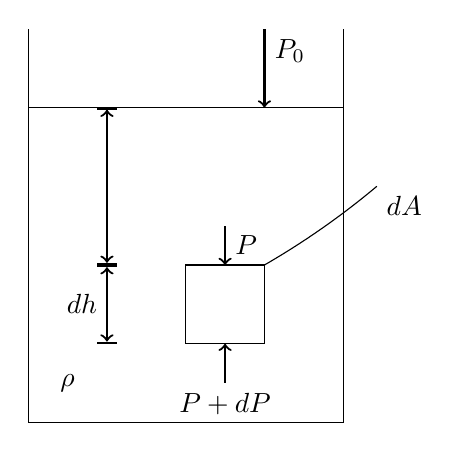
\begin{tikzpicture}
    \draw (0,0) rectangle (4,4);
    \draw (0,4) -- (0,5);
    \draw (4,4) -- (4,5);
    \draw[thick, <-] (3,4) -- (3,5) node[anchor=north west]{$P_0$};
    \draw (2,1) rectangle (3,2);
    \draw[thick, <-] (2.5,2) -- (2.5,2.5) node[anchor=north west]{$P$};
    \draw[thick, <-] (2.5,1) -- (2.5,0.5) node[anchor= north]{$P+dP$};
    \draw (0.5,0.5) node{$\rho$};
    \draw (3,2) arc (300:310:10cm) node[anchor=north west]{$dA$};
    \draw[thick, |<->|] (1,4) -- (1,2);
    \draw[thick, |<->|] (1,2) -- (1,1);
    \draw (1,1.5) node[anchor=east]{$dh$};
    \end{tikzpicture}
    \caption{Tank and pressure}
    \label{fig:tank}
\end{figure}